\documentclass[letterpaper,12pt]{article}
\usepackage[utf8]{inputenc}
\usepackage{fullpage}
\usepackage{courier}
\usepackage[margin=0.75in]{geometry}
\usepackage{listings}
\usepackage{color}
\usepackage{graphicx}
\usepackage[width=5in]{caption}
\usepackage{hyphenat}
\usepackage[section]{placeins}
\usepackage{cmll}

% Format a sectionless paragraph
\newcommand*\unparagraph{
	\par
	\nopagebreak
	\vskip3.25ex plus1ex minus.2ex
	\noindent
}

% define extra colors
\definecolor{dkgreen}{rgb}{0,0.6,0}
\definecolor{purple}{RGB}{159,0,197}

% define the code listing format
\lstset{
	language=C++,
	basicstyle=\footnotesize\ttfamily,
	backgroundcolor=\color{white},
	showspaces=false,
	showstringspaces=false,
	frame=none,
	tabsize=3,
	keywordstyle=\color{purple},
	commentstyle=\color{dkgreen},
	stringstyle=\color{blue},
	escapeinside={\%*}{*)}
}

% define the title/header
\title{\Large CS 1428 Honors\\Lab 3}
\author{Jared Wallace}
\date{}

\begin{document}

\maketitle

\vspace{30mm}

\section*{Questions}

\begin{enumerate}
    \item (15 pts) Write a simple program that functions as a basic exponentiation tool.
          You should prompt the user for both a number and the power to raise it to.
          Then the program should calculate and output to stdout the result. Name
          your program lab3h\_part1.cpp
    \item (25 pts) If you did not use a switch statement last week in your calculator program,
          convert it now so that it does. Ensure your program continues to meet all
          requirements after conversion. Name your program lab3h\_part2.cpp
    \item (60 points) Create a program named lab3h\_part3.cpp that functions as a number guessing game.
          Requirements:
            \begin{itemize}
                \item You should prompt the user for the range they wish to be guessing from, ie. 1-10.
                \item The user should be prompted to input the high and low limits as separate integers.
                \item The game should then begin, and the user should be prompted for their first guess.
                \item The user will submit their guess and one of four things should happen:
                    \begin{enumerate}
                        \item The guess is correct – output a statement informing them they guessed
                              correctly as well as the number of tries it took them to get it right.
                        \item The guess was too low – output a statement indicating that the guess
                              was incorrect and inform them that the guess was too low.
                        \item The guess was too high – output a statement that the guess was incorrect
                              and inform them them that the guess was too high.
                        \item The guess was out of range – output a statement that the guess was out
                              of range and inform them of the correct range.
                    \end{enumerate}
                \item At the end of the game, ask the user whether or not they want to play again.
                      If they do, start the game over again.
                \item For this program I have supplied a starter file to handle the random number
                      generation. You MUST use this file in order for your program to work correctly.
                      ( unless you really want to show off )
            \end{itemize}
\end{enumerate}
\section*{Deliverables}
Hard copy of the source code you wrote (lab2h\_part1.cpp, lab2h\_part2.cpp, and lab2h\_part3.cpp)
and the answers to the questions. Soft copy (upload to homework upload) of all your source code files.

% Comic at the bottom
\begin{figure}[ht!]
	\centering
	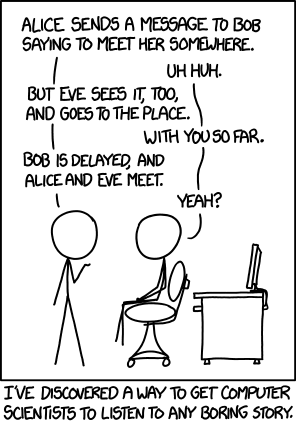
\includegraphics[width=3in]{protocol.png}
    \caption*{Changing the names would be easier, but if you're not comfortable lying, try only making friends with people named Alice, Bob, Carol, etc.}
\end{figure}
\end{document}
